\section{Background and Motivation}

In this section, we provide the background and motivation for this work.

\subsection{Graph Vertex Processing}

\begin{figure}[htbp]
\centering
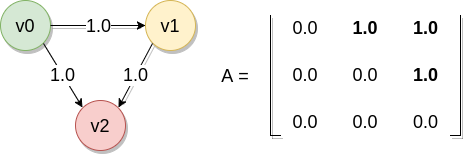
\includegraphics[width=0.5\textwidth]{figures/sample_graph}
\caption{Sample Graph Representation}
\label{fig:sample_graph}
\end{figure}

\begin{figure}[ htbp ] 
\begin{equation}
\#Edges = A^{T} \times Identity
\end{equation}
\begin{equation}
\#Edges = 
\left(\begin{array}{ccc} 0 & 0 & 0 \\ 1 & 0 & 0 \\ 1 & 1 & 0 \end{array}\right) \times
\left(\begin{array}{c} 1 \\ 1 \\ 1 \end{array}\right) 
= \left(\begin{array}{c} 0 \\ 1 \\ 2 \end{array}\right) 
\end{equation}
\caption{Incoming Edges Algorithm}
\label{fig:sample_algorithm}
\end{figure} 

\begin{lstlisting}[emph={Assign, Process, Apply}, emphstyle=\color{blue}, numbers=none, escapechar=\%, caption=Graph Vertex Processing Model]
GraphProgram(%\textit{G}%, %\textit{P}%, %\textit{N}%) :
  for_each %\textit{N}% :
    x := Assign(%\textit{P}%)
  	y := Process(%\textit{G}%,x)
  	%\textit{P}% := Apply(%\textit{P}%,y)	  
  
e.g. FindIncomingEdges(%\textit{G}%=A, %\textit{P}%=%\textit{\textbf{I}}%, %\textit{N}%=1) :
           Assign(%\textit{P}%)    := %\textit{P}%
     where Process(%\textit{G}%,x) := %\textit{G}% * x
           Apply(%\textit{P}%,y)   := y
\end{lstlisting}

A large variety of programming models have been proposed for describing Graph algorithms, expressing computation using vertex operations on matrices \cite{GraphMat} \cite{GraphLab}, \cite{Pregel}, \cite{MapGraph} \cite{GraphX} task-based models \cite{Galois} or domain-specific languages \cite{GreenMarl}. The vertex programming model has show great adoption for its ease of abstraction for describing algorithms using Linear Algebra and its efficient computation on commodity multi-core processors.

Figure \ref{fig:sample_graph} shows a simple 3 vertices graph example with its corresponding 3x3 matrix representation. For every edge between a source and destination vertex, the corresponding row and column entry in the matrix is activate. For instance, the matrix entry in row 0 and column 1 represents the edge between source \textit{v0} and destination \textit{v1}. using the matrix representation, we can apply an algorithm on the graph to calculate the total number of incoming edges at each vertex. This algorithm can be expressed using a simple matrix-vector operation as shown in equations (1) and (2) in Figure \ref{fig:sample_algorithm}. Several graph algorithms, including Breadth First Search (BFS) \cite{BFS}, PageRank \cite{PageRank}, Single Source Shortest-Path (SSSP) \cite{SSSP}, can be described similarly using the vertex programming model \cite{GraphMat}.

Listing 1 shows the three stages of a generalized graph vertex processing model - \textit{Assign}, \textit{Process} and \textit{Apply}, given a graph \textit{G}, some vertex properties \textit{P} and an iteration count \textit{N}. The \textit{Assign} stage generates an input vector \textit{x} using the vertex properties \textit{P}. The \textit{Process} stage applies the input vector \textit{x} to the graph \textit{G} and generates an output vector \textit{y}. The\textit{ Apply} gather the resulting output vector to update the vertex properties for the next iteration. The graph program executes the three stages for several iterations until it converges. A direct mapping of our incoming edges algorithm to this processing model is also provided in Listing 1, where the identity vector is used for the vector properties. The \textit{Assign} and \textit{Apply} stages of this program are simple identity operators, while the \textit{Process} stage perform a matrix-vector multiplication. The input graph can be represented as a compressed sparse matrix to only store the non-zero entries of the graph. This data structure enables accelerated computation, often using a Sparse Matrix-Sparse Vector Multiplication (SpMSpV) kernel to target multi-core CPUs \cite{GraphMat} or GPUs \cite{MapGraph}. The computation that cannot be accelerated is simply executed on the general-purpose host CPU. FlexGraph's objective is to provide a more energy efficient graph processing backend using a FPGA for hardware acceleration \cite{Catapult}.

\subsection{Intel Heterogeneous CPU-FPGA Platform}

\begin{figure}[htbp]
\centering
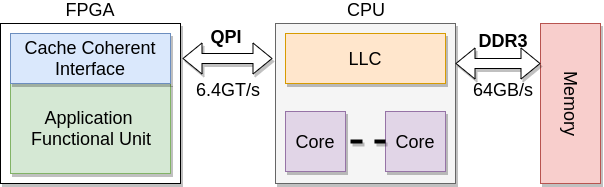
\includegraphics[width=0.5\textwidth]{figures/harp_arch}
\caption{Intel HARP Architecture}
\label{fig:harp_arch}
\end{figure}

\begin{figure*}
\centering
\begin{subfigure}{0.4\textwidth}
    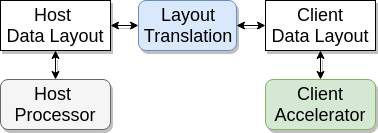
\includegraphics[width=\textwidth]{figures/offload_model}
    \caption{Offload model}
    \label{fig:offload_model}
\end{subfigure}
\hfill
\begin{subfigure}{0.4\textwidth}
    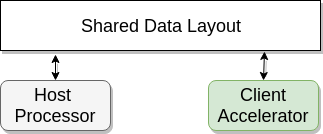
\includegraphics[width=\textwidth]{figures/collaborative_model}
    \caption{Collaborative model}
    \label{fig:collaborative_model}
\end{subfigure}
\caption{Shared Memory Compute Models}
\label{fig:compute_model}
\end{figure*}

With the rising adoption of FPGAs in production data centers \cite{Catapult}, there is a need to increase its ecosystem by making them more energy efficient as well as accessible to both the users and designers. Modern CPU-FPGA platforms \cite{CPU-FPGA} provide tightly-coupled shared-memory CPU-FPGA integration \cite{CAPI} \cite{CCI}, making then easier to program and efficient for hardware acceleration. Figure \ref{fig:harp_arch} shows an overview architecture of the Intel Xeon-FPGA platform prototype that we used in our evaluation. It has a dual-socket system, one containing a 10-core Intel Xeon E5-2680 CPU and the other containing an Altera Stratix V 5SGXEA FPGA operating at 200 MHz. The two sockets are connected via a 6.4 GT/s QPI \cite{QPI} link for data transfer. The FPGA's area is partitioned into two main blocks - the Application Function Unit (AFU) or 'Green' bitstream allocated for the custom accelerator and the 'Blue' bitstream implementing the Cache Coherent Interface (CCI) for the accelerator. The CCI runtime implements a 64 KB direct-mapped cache to support address translation (1024 page table entries) with request re-ordering for a total of 2 GB of addressable memory. The AFU memory interface is 64-byte cache-line addressable and it is up to the accelerator to extend the interface if fine grained (e.g. single byte) access is desired.

\subsection{Collaborative CPU-FPGA Computation}

The prevalent execution model for accelerator design is the offload model \cite{Accelerators} where computation takes place on discrete copies of a shared resource that are optimized for efficient access by the target device. In this model of computation, the host processor applies some layout translation on the data before making it available to the client accelerator (see Figure \ref{fig:offload_model}). The additional latency of the translation process is generally mitigated using optimization techniques such as batching and double-buffering. The offload model is well suited for discrete memory systems where the necessary data transfer can be coupled with layout translation. One attractive application of shared-memory systems is the enabling of efficient collaborative computation (see Figure \ref{fig:collaborative_model}) in which all attached compute elements can access the same shared resource and modifying it during the course of the program execution. It is particularly ideal if the data layout provides efficient access by the compute devices. Contrarily to existing Graph Analytics Accelerators \cite{Graphicionado} \cite{GraphOps} that employ a custom optimized graph data structure for computation, Flexgraph uses a sparse matrix format for computation. This decision provides several advantages - first, it is storage efficient because the graph's physical memory is shared - second, it enables collaborative computation with the host CPU, leveraging the large ecosystem of matrix-based frameworks \cite{CombBlas} \cite{Pegasus} - third, it decouples the software and hardware design, enabling them to scale independently.

\section{FlexGraph Architecture}

In this section, we describes the overall architecture of the FlexGraph Accelerator.

\subsection{The DCSC Matrix Format}

\begin{figure}[htbp]
\centering
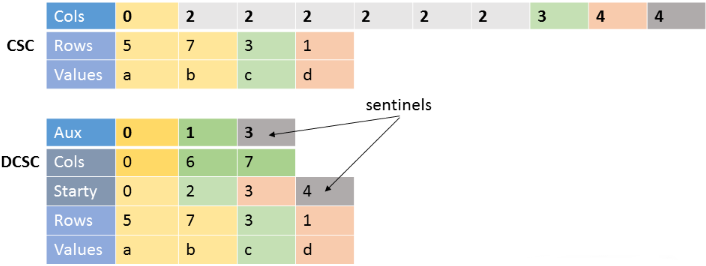
\includegraphics[width=0.5\textwidth]{figures/DCSC_matrix_format}
\caption{DCSC hyperspace matrix format}
\label{fig:DCSC_matrix_format}
\end{figure}

FlexGraph uses the Doubly Compressed Sparse Column (DCSC) \cite{DCSC} format as underlying graph data structure. The format allows minimal traversal into the sparse matrix structure, saving necessary memory bandwidth when fetching empty columns. Figure \ref{fig:DCSC_matrix_format} shows a sample matrix A = \{(0,5,a), (0,7,b), (6,3,c), (7,1,d)\} with four non-zero edges (src, dst, weight) encoded using DCSC versus the conventional CSC \cite{CSC} format. The traversal over CSC requires accessing all consecutive column ranges \textit{(cols[i+2] - cols[i])} even though most of the distances are empty. DCSC saves on bandwidth by using an additional indirection  buffer inside its structure to only encode non-zero columns. It is important to note that this indirection can introduce additional storage overhead and access latency if the matrix is too small or not sparse enough. However, Graph Analytics datasets are generally very large and hyper-sparse which eliminate the DCSC format overhead. In addition to a sparse matrix, FlexGraph also uses a sparse vector to provide property data as well as edge selection during computation. A bitmask is used to encode the non-zero entries in the input vector.

\subsection{The Sparse Matrix-Sparse Vector Multiplication Kernel}

FlexGraph micro-architecture implements a Sparse Matrix-Sparse Vertex Multiplication (SpMSpV) kernel in FPGA. This kernel diverges from conventional Sparse Matrix-Vector Multiplication (SpMV) implementations in two ways - firstly, it uses a sparse data structure as input and output vector during computation - secondly, it uses a doubly-compressed sparse matrix (DCSC) format with additional memory indirection buffer when accessing the matrix columns. These two properties present unique performance challenges when designing the accelerator. Listing 1 shows the pseudo-code of the SpMSpV kernel. Given the start/end addresses (col\_start, col\_end) into the matrix columns buffer (coldata), for The program iterates through each column entry and fetches the corresponding column index (col) and rows buffer address (row\_start, row\_end). It then checks if the current column index (col) is active using the vertex bitmask, only then it proceeds with rows traversal loop where the matrix row\_data is accessed to retrieve corresponding row index and matrix value for computation. A Multiply-Accumulate (MAC) operation is then performed on the matrix and vertex data and output bitmask is updated. Lines 6 and 8 show the code region where external memory is randomly accessed to obtain the vertex data and active state. Lines 5 and 10 show the code region where external memory is accessed semi-random because only the first access cannot be predicted and after that the address is simply incremented. FlexGraph's architecture attempts to address some of those performance hogs using several optimizations detailed in section 4.

\begin{lstlisting}[
	linebackgroundcolor={
	\ifnum\value{lstnumber}=6\color{red!10}\fi
	\ifnum\value{lstnumber}=8\color{red!10}\fi
	\ifnum\value{lstnumber}=5\color{orange!10}\fi
	\ifnum\value{lstnumber}=10\color{orange!10}\fi}, 
        escapechar=\%, 
        emph={col_start, col_end, coldata, rowdata, values, active}, emphstyle=\color{blue}, language=Python, caption=Pseudo-code for SpMSpV kernel]
def SpMSpV_kernel(a, x):
  y_values[] = {0}
  y_bitmask[] = {false}
  for i in (a.col_start, a.col_end):            	
    (col, row_start, row_end) = a.coldata[i]
    x_active = x.bitmask[col]          
    if (x_active) :                            
      x_value  = x.values[col]              
      for j in (row_start, row_end): 
        (row, a_value) = a.rowdata[j]
        y_values[row] += a_value * x_value
        y_bitmask[row] = true          
  return (y_values, y_bitmask)
\end{lstlisting}

\subsection{FlexGraph Microarchitecture}

Externally, FlexGraph input and output signals implement an Accelerator Functional Unit (AFU) interface defined by Intel's Accelerator Abstraction Layer (AAL) \cite{Intel-FPGA}. AFUs implementing the interface are able to bind with the FPGA's board support package (BSP) and seamlessly communicate with the AAL software running on the host processor. Listing 2 shows AAL device interface implementation using Cocoh's API. Our FlexGraph Accelerator's class in Cocoh simply derives from this interface and override the \textit{initialize()} function to provide its implementation and Cocoh takes care of generating the corresponding verilog module. It implements three input signals \textit{(start, qpi\_in, ctx)} and two output signals \textit{(qpi\_out, done)}. The AFU starts execution when the \textit{start} signal is asserted and communicate completion by asserting the \textit{done} signal. The \textit{ctx} signal provides application's specific data like constants and buffers address in the case of FlexGraph. The \textit{qpi} in/out signals implement Intel Quick Path Interconnect (QPI) interface \cite{QPI}, providing single channel read/write ports for accessing external shared memory. The FPGA socket hosts a 64-byte cache coherent interface (CCI) \cite{CCI} that connects to the host processor's last level cache (LLC) via QPI.     

\begin{lstlisting}[language=C++, caption=AAL Device Interface in Cocoh C++]
class aal_device {
public: 
  virtual out_t initialize()(
    const ch_logic& start, 
    const qpi::in_t& qpi_in, 
    const afu_ctx_t& ctx, 
    qpi::out_t& qpi_out, 
    ch_logic& done
  ) const = 0;  
};
\end{lstlisting}

\begin{figure}[htbp]
\centering
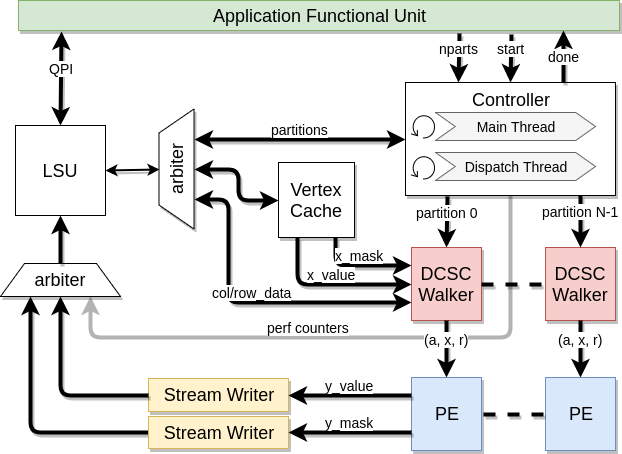
\includegraphics[width=0.4\textwidth]{figures/microarchitecture}
\caption{FlexGraph Microarchitecture}
\label{fig:microarchitecture}
\end{figure}

Figure \ref{fig:microarchitecture} illustrates FlexGraph accelerator microarchitecture. It is comprised of four main module types, a controller, processing elements (PEs), a load store unit (LSU) and vertex caches. The main controller is responsible for starting the accelerator, scheduling tasks for execution, reporting hardware counters and terminating the execution. The processing elements execute partition tasks assigned to them by the controller and communicate with the LSU to access the matrix and vertex data for their partition. They are also responsible for sending their final output result back to memory. The LSU is the module responsible for managing external communication between the accelerator and memory via the QPI interface. It directly binds to the QPI ports defined in listing 2.
The vertex caches store intermediate vertex data and active masks for sharing between the processing elements. FlexGraph processing pipeline sightly resembles the SPMV execution steps illustrated in listing 1. We made several important modifications to it to improve performance.  

\section{FlexGraph Optimizations}

The first optimization we performed in FlexGraph early during the design phase was the support of multiple processing units. The reasoning behind it was to extract the maximum bandwidth out of the LSU such that the QPi is always busy processing a request when some processing element are stalled waiting for their data to return. the other advantage of parallelization for FlexGraph is to increase the overall accelerator throughput by processing multiple a larger chunk of the workload per unit of time. The scheduling of the partitions for execution on the processing elements is controlled by a dispatch unit inside the main controller module. The dispatch unit fetches partitions data from the LSU and pass down each partition in a first come first serve fashion to the processing elements.

\subsection{DCSC Matrix partitioning}

\begin{figure}[htbp]
\centering
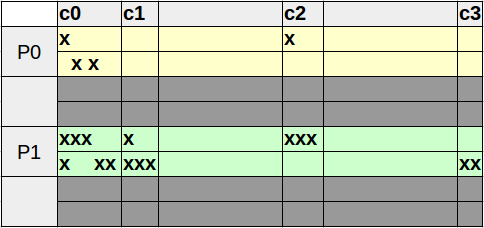
\includegraphics[width=0.4\textwidth]{figures/matrix_partitioning}
\caption{DCSC Matrix Partitioning}
\label{fig:matrix_partitioning}
\end{figure}

To enable the parallelization of FlexGraph tasks, the DCSC sparse matrix is first partitioned into aligned partitions of 32 consecutive rows containing non-zero edges. we choose a partition size of 32 mainly to match the 32-bit size of the bitmasks encoding the vertices that are active. These masks are used by the software on the host processor to determine the regions of the acceleration's output buffer that have been updated. Figure \ref{fig:matrix_partitioning} illustrates sample matrix partitioning in which the non-zero horizontal regions have been broken into two partitions P0 and P1. The non-zero column ranges \textit{(c0, c1, c2, c3)} represent the selected chunks covered by each partition. Partition P0 will only contain ranges \textit{c0} and \textit{c2} while P2 has non-zeros in all four ranges. The partitioning scheme is not ideal because of the workload in-balance that might exist when the number of non-zero varies disproportionally between partitions.  

\subsection{Synchronising Memory Accesses}

\begin{figure}[htbp]
\centering
\includegraphics[width=0.35\textwidth]{figures/write_masks_synchronization}
\caption{Active Masks Write Synchronization}
\label{fig:write_masks_synchronization}
\end{figure}

An implementation challenge we faced when supporting multiple processing elements in FlexGraph was the synchronization of write accesses for the output active masks. Because the LSU data transfer granularity is 64 byte (matching CCI \cite{CCI}), FlexGraph need to manage shared write accesses to the same block to avoid having a processing element override the content of another one. Luckily this doesn't pose any problem for writing out partition output values because the 32 rows within a partition occupy 32 * 4 bytes = 2 x 64 bytes blocks. Because the partitioning reinforces 32 rows alignment, each processing element can safely write into their assigned blocks. However, writing out the active masks poses a challenge because a single 4-byte mask encodes the active states of all 32 rows in a partition. This causes the processing elements to potentially share a single 64-byte block when writing the masks out to memory. To alleviate the contention, FlexGraph keep N active 64-byte blocks locally assigned to either one of the N processing elements. It assigns an ownership bit mask to each block to track their reference count and the processing element assigned to them. It also tracks the current address value assigned to each block. When a processing element is ready to write its 4-byte active mask, it passes the mask address and value to the LSU. The LSU goes to last active block the processing element previous wrote to and check if the block address matches. If so, it simply adds the new content to the existing block. If there is no match, it clears its ownership bit and flushes the block to memory if the ownership mask goes to zero. Then it looks up the other active block if anyone already has the address to use it, otherwise if it acquires the last unused block. Figure \ref{fig:write_masks_synchronization} shows a simplified illustration of the scheme with two processing elements. We don't need to keep more than N blocks in local storage for this scheme to work because the block address references are always incremental and never regress, meaning that there is always going to be free block available to use. It is important to also point out that for this scheme to work, the operation has to be atomic. FlexGraph has a single communication channel between all processing elements and the LSU which does some round robin arbitration and blocks the write mask request until it is committed. We also investigated an alternative solution to avoid this synchronization, which is simply increasing the partition size to 16 * 32 rows, allowing the aggregated active masks to occupy a full 64-byte block. They were two major issues with this approach. Firstly, the total size of all resident partitions will be too large if we support multiple processing elements. Secondly, it will worsen the workload imbalance that is already present with 32 rows.     

This section describes some optimizations we added to FlexGraph to improve its performance. 

\subsection{Optimizing Memory Accesses via Stream Buffers}

\begin{figure}[htbp]
\centering
\includegraphics[width=0.4\textwidth]{figures/stream_buffers}
\caption{Stream Buffers}
\label{fig:stream_buffers}
\end{figure}

As stated before, FlexGraph's LSU transfer granularity is 64 bytes, which is much larger than the 4 bytes of elements accessed by the processing elements. To save on bandwidth, the LSU uses stream buffers that fetch a 64-byte blocks of data but extracts 4-byte elements at the time. It is implemented using a fifo structure in the back-end where 64-byte responses from QPI go
 into. In the front-end, there is a temporary 64-byte block that is extracted from the fifo on demand to deliver 4-byte element at the time. We employ a shift register to extract the 4-byte element to pass it to the processing element. Figure \ref{fig:stream_buffers} shows an illustration of the stream buffer concept.
   
\subsection{Caching Vertex Values and Masks}

Another optimization we implemented in FlexGraph is the caching of vertex values and masks. Looking at the SPMV speudo-code in listing 1, we can observe in lines 5 and 6 that there is a random memory access to buffers \textit{x\_values} and \textit{x\_activemask}. FlexGraph employs a stream buffer like concept to consume 64-byte vertex data once they arrive inside the processing element to each iteration loop. However, the same block can be referenced by another processing element and sharing them inside the cache structure can save unnecessary memory traffic. We implemented two small fully associative caches with first-in-First-out replacement to hold active vertex data during execution. The caches are implemented inside the LSU which is responsible for managing them. When a vertex request arrives from a processing element, the LSU first looks up the cache if the block is already present and return it. If the block is not there, it sends the request to QPI. QPI output interface support a 14-bit metadata field that is used to identify the block once it is returned. We use that field to store the index of the block such that we can compute the cache tag when it arrives. Because the cache is small, we implemented a one cycle tag lookup for the LSU to known if the block is present and accessible.

\subsection{Executing Non-blocking Memory writes}

FlexGraph memory writes are all non-blocking, this applies to both the output values and active masks. This allows the processing elements to push their write request and resume execution while the LSU is processing them. Upon write responses from the QPI channel, the LSU internally keeps track of the count of outstanding requested to ensure that all writes have completed. The QPI interface exposes two write response ports by which the memory replies could be sent. This allows servicing two responses simultaneously. The LSU implements a mechanism to process both channels simultaneously when they are active. At completion time when all processing elements are done executing the current run, the controller waits for all outstanding write requests to complete before asserting the \textit{done} signal.

\section{FlexGraph Software-Hardware Codesign}